%% cycle4_ar_tr.tex
%
%  Spitzer Space Telescope Cycle-4 Proposal Template
%
%  Use this template for Archival Research or
%  Theoretical Research proposals.  No style file is required.
%
%  Version 1.0    16 October 2006
%
%%%  For Spitzer proposal preparation resources please visit 
%    the proposal kit web page: 
%
%%%  http://ssc.spitzer.caltech.edu/propkit/ 
%
%  **In particular, please read the Cycle-4 Call for Proposals (CP).
%  **It is the definitive document that describes the requirements
%  **necessary for your proposal.
%
%    Please address all questions regarding the proposal 
%    and observation to the Helpdesk at 
%
%%%  help@spitzer.caltech.edu
%
%
%
%%%%%%%%%%%%%%%%%%%%%%%%%%%%%%%%%%%%%%%%%%%%%%%%%%%%%%%%%%%%%%%%%%%%%%%%
%
%  The template begins here.  The font must be 12 point and the margins
%  must be at least 1-inch on all sides. 
%  Don't override this.  
%
% If you compile this and find that the text is "mushed up against
% the top of the page", the default paper size for your installation 
% of latex is A4.  In order to override this, do:
% > latex texfile # where the manuscript is in a file named texfile.tex
% > dvips -Ppdf -t letter -o texfile.ps texfile
% finally, to get nice (non-blurry, searchable) pdf do:
% > ps2pdf13 texfile.ps  texfile.pdf
% if you do not have ps2pdf13, please ask your sysadmin to install it.


\documentclass[letterpaper,12pt]{article}
\usepackage{epsfig,colortbl}
\textwidth=6.5in
\textheight=9.5in
\topmargin=-0.75in
\oddsidemargin=0.0in
\evensidemargin=0.0in
\pagestyle{myheadings}
\parindent=0in
\usepackage{subfigure}

% Please update the following line with the title of your proposal
% and your Author name (with "et al." if more than two authors).

\markright{Spitzer SINGS a SONG, G.\ Brunner et al.}
\pagenumbering{arabic}

\begin{document}

\section{Scientific Justification}

\subsection{Spitzer SINGS a SONG of Galactic Evolution}

\indent Galactic evolution is inherently correlated with molecular gas within a galaxy.  In the Milky Way Galaxy, we observe molecular gas in dense molecular clouds.  The collapse of these molecular clouds triggers a burst of star formation.  In other galaxies, we observe molecular gas trigger star formation in spiral arms via the passage of a spiral density wave (Vogel et al. 1983), within nuclear regions of galaxies (Young and Deveraux 1991), and at the ends of bars in barred spiral galaxies (Sheth et al. 2000).  Thus, molecular gas serves as the fuel for star formation and is fundamentally connected with galaxy evolution.\\

% through a variety of processes.

Prior to the Infrared Space Observatory (ISO) and the Spitzer Space Telescope (Spitzer), much of our knowledge of the conditions of the molecular gas in galaxies came from studies of CO emission.  CO (J = 1 - 0) emission directly traces the mass of the coldest (T = 5 - 10 K) molecular hydrogen ($\mathrm{H_2}$) within galaxies.  Spitzer has given us access to the lowest pure rotational levels of $\mathrm{H_2}$.  The $\mathrm{H_2}$(0-0)S(0) (28.2 $\mu$m) and $\mathrm{H_2}$(0-0)S(1) (17.1 $\mu$m) lines can both be observed with the Spitzer IRS long-low (LL) modules (14 - 38 $\mu$m, with LL1 covering 14 - 21 $\mu$m and LL2 covering 21 - 38 $\mu$m).   These lines trace the warm (T = 100 - 300 K) molecular gas.\\

The $Spitzer$ $Infrared$ $Nearby$ $Galaxies$ $Survey$ (SINGS) legacy program has surveyed 75 nearby galaxies (Kennicutt et al. 2003).  These galaxies range in Hubble type, luminosity, star formation, and nuclear activity.  The SINGS legacy has used the Spitzer IRS LL (LL1 and LL2)  module in spectral mapping mode to map radial strips across 65 galaxies within their sample.  The radial strips cover a range of dynamically distinct regions within galaxies (i.e. nuclei, spiral arms, HII regions, etc.).  The strips are roughly 50 x 600 arcsec in area and give us spatially resolved spectra across the galaxies.  {\bf These strips contain a wealth of data.}    In addition to observing $\mathrm{H_2}$ S(0) and $\mathrm{H_2}$ S(1) in the LL strips, there are a atomic features ([NeIII] (15.55 $\mu$m), [SIII](18.71 $\mu$m), [FeII](25.83 $\mu$m), [OIV](25.89 $\mu$m), [SIII](33.48 $\mu$m), and [SiII](34.82 $\mu$m) and broad PAH complexes  at 16.4 $\mu$m and 17 $\mu$m (Smith et al. 2004).\\

While the SINGS team is currently studying the $\mathrm{H_2}$ lines (Roussel et al. 2007, in preparation), {\bf they have only done so for the nuclear regions} of the SINGS sample.  Their study of the $\mathrm{H_2}$ uses aperture averaged spectra over the nuclei  of the 65 galaxies to determine the excitation-temperature, mass, and ortho-to-para ratio (OPR) of $\mathrm{H_2}$ within the galaxies.  Their study {\bf does not} explore $\mathrm{H_2}$ outside of the nuclei of the galaxies and they {\bf do not} take advantage of the spatial resolution of the spectra across the galaxy.\\

{\bf We propose to take full advantage of the spectacular SINGS IRS LL coverage across the nuclear regions and disks in order to understand the spatial distribution of the warm (T = 100 - 300 K) $\mathrm{H_2}$ across a sample of 18 galaxies that have been observed by both SINGS and the  Berkeley-Illinois-Maryland-Array Survey of Nearby Galaxies (BIMA SONG) (Regan et al. 2001, Helfer et al. 2003)}.  The 18 galaxies (listed in table 1) have been studied as part of BIMA SONG and have CO (J = 1 - 0) maps publicly available on the NASA extragalactic database (NED).  CO (J = 1 - 0) emission traces the cold (T = 5 - 10 K) $\mathrm{H_2}$ and the maps allow us to understand the spatial distribution of the cold $\mathrm{H_2}$ mass.  We will use the SINGS LL data cubes to map the $\mathrm{H_2}$ S(0) and $\mathrm{H_2}$ S(1) lines across the galaxies.  From these lines will will determine the warm $\mathrm{H_2}$ mass and temperature distributions across the galaxies.  We will correlate the cold $\mathrm{H_2}$ (traced by CO emission) with the warm $\mathrm{H_2}$ (traced by the $\mathrm{H_2}$ S(0) and $\mathrm{H_2}$ S(1) emission) in order to understand the relationship between the warm and cold $\mathrm{H_2}$.  Additionally, we would like to understand the connection between $\mathrm{H_2}$ (both the cold and warm phases) and the mid-infrared spectral diagnostics (17 $\mu$m PAH feature, [NeIII] (15.55 $\mu$m), [OIV](25.89 $\mu$m) as a shock tracer, and electron density determined by [SIII](33.48 $\mu$m)/[SIII](18.71 $\mu$m)) that we can also map from the SINGS LL data cubes.\\

We have used IRS spectral mapping data acquired though GO - 20138 (PI: K. Sheth) of M51a (the Whirlpool galaxy, NGC 5194) as a test case for our study (Brunner et al., submitted).  In working with M51a, we have created a data analysis pipeline that takes IRS SL and LL data cubes and creates extinction corrected line flux maps.  Our pipeline utilizes PAHFIT (Smith et al. 2007) to decompose mid-infrared spectra across the LL data cubes.  These maps are powerful tools for understanding the spatial variation of $\mathrm{H_2}$ and other mid-infrared spectral lines.\\

For M51a, we had both SL and LL coverage of an overlapping strip across M51a.  We have used our pipeline to map $\mathrm{H_2}$ S(0), $\mathrm{H_2}$ S(1) (both lines in LL), $\mathrm{H_2}$ S(2), $\mathrm{H_2}$ S(3), $\mathrm{H_2}$ S(4), and $\mathrm{H_2}$ S(5)  (all four lines in the SL).  Figure 1 shows the maps of the $\mathrm{H_2}$ S(0) and $\mathrm{H_2}$ S(1) emission across M51a.  We have used these lines to understand the temperature and mass distribution of the warm $\mathrm{H_2}$ across M51.  In figure 2, we show the warm mass distribution compared to the warm $\mathrm{H_2}$ temperature distribution.  We find that the $\mathrm{H_2}$ is warmest within the center of the galaxy and is coolest in the spiral arms (which contain the bulk of the $\mathrm{H_2}$ mass).  We also compared the cold $\mathrm{H_2}$ to the warm $\mathrm{H_2}$.  In the inner spiral arms, we see offsets in the location of the peak emission within the spiral arms.  Why is this?  Additionally, we are able to map $\mathrm{H_2}$ excitation-temperature and mass in spiral arms out to 7 kpc from the nucleus of the galaxy.  The SINGS LL strip cover a much greater distance in the galaxy allowing us to understand how excitation-temperature and $\mathrm{H_2}$ mass vary as a function of galactocentric radius.\\

We have also studied the ortho-to-para ratio (OPR) across M51a.  From our study we found that the lower pure rotational levels ($\mathrm{H_2}$ S(0), $\mathrm{H_2}$ S(1), $\mathrm{H_2}$ S(2), and $\mathrm{H_2}$ S(3)) exhibit an OPR of 3 (or very close to) in the nuclear and spiral arm regions.  Under the assumption that the OPR is 3 across the galaxies, we can map the warm $\mathrm{H_2}$ excitation-temperature and $\mathrm{H_2}$ mass across the 18 galaxies that we would like to study.\\

For galaxies observed by both SINGS and SONG we would like to address the following questions:\\

{\bf 1. How does the warm (T = 100 - 300 K) $\mathrm{H_2}$ temperature and mass vary across dynamically distinct regions within galaxies?}  The majority of the $\mathrm{H_2}$ mass radiates in the lower energy level $\mathrm{H_2}$ lines.  In mapping the $\mathrm{H_2}$ S(0) and $\mathrm{H_2}$ S(1) lines across the LL strips we can determine the $\mathrm{H_2}$ excitation-temperature and mass distributions across the galaxies (Rigopoulou et al. 2002, Higdon et al. 2006). This will allow us to undertand how the $\mathrm{H_2}$ temperature and mass varies between the nucleus, spiral arms, and inter-arm regions within the galaxies. We will determine the fraction of warm $\mathrm{H_2}$ that is found in the nucleus of the galaxies and  the fraction that is found in the disk and spiral arms.  We will also determine how the excitation-temperature and mass changes in spiral arms as a function of galactocentric radius.\\

{\bf 2.  How do the warm and cold $\mathrm{H_2}$ correlate across dynamically distinct regions in galaxies?}  Are there offsets in the location of the warm and cold $\mathrm{H_2}$?  If so, why?  The combination of CO data and the $\mathrm{H_2}$ lines for every galaxy will allow us to correlate the different molecular gas phases.  We find that in M51a, the warm and cold $\mathrm{H_2}$ are offset in different regions.  Do we observe offsets in the location of warm and cold $\mathrm{H_2}$ in other galaxies?  What does this mean?\\ 

{\bf 3.  How does the warm and cold $\mathrm{H_2}$ mass correlate with the mid-ifrared spectral diagnostics?}  The [OIV](25.89 $\mu$m) line has been observed to arise from shocks, the stellar winds of Wolf-Rayet stars, high-mass star photoionization, and active galactic nuclei (Schaerer and Stasinska 1999, Lutz et al. 1998, Smtih et al. 2004).  With PAHFIT, we are able to de-blend the [FeII](25.99 $\mu$m) and [OIV](25.89 $\mu$m) lines.  This allows us to discern regions where shocks are exciting the ISM.  If we observe [OIV](25.89 $\mu$m) emission coinciding with $\mathrm{H_2}$, this would imply that the $\mathrm{H_2}$ is excited by shocks.  We will use our ability to spatially resolve the mid-infrared emission features to discern the excitation mechanism of warm $\mathrm{H_2}$ in dynamically different regions of the galaxies.\\

Additionally, the ratio of the [SIII](33.48 $\mu$m) and [SIII](18.71 $\mu$m) lines provide a determination of the electron density in HII regions.  Comparison to the $\mathrm{H_2}$ data will allow us to determing the location of cold and warm $\mathrm{H_2}$ to the hot ionized gas in HII regions.  This will allow us to understand the relationship of the hot ionized gas and and the warm and cold molecular gas within the spiral arms of galaxies.\\

The comparison of $\mathrm{H_2}$ emission to other mid-infrared spectral diagnostics will allow us to understand the conditions of the ISM across galaxies and the processes that excite the ISM.  In figure 3, we present maps of $\mathrm{H_2}$ S(0), $\mathrm{H_2}$ S(1), [OIV](25.89 $\mu$m), [SIII](33.48 $\mu$m), and [SIII](18.71 $\mu$m) from M51a.\\

\clearpage

\section{Technical Plan}

%{\bf Data Reduction:} We will construct data cubes from the IRS observations using CUBISM (citation).  Both the PI (Brunner) and Co-I (Sheth) are experts with the CUBISM software.  The PI will be responsible for producing data cubes of the galaxies.  CO maps from the BIMA survey are already reduced and they are science ready.\\

The SINGS legacy has provided IRS low resolution data cubes for 65 galaxies.  As of data release 4 (DR4), there are 16 galaxies observed by SONG that have publicly available SINGS low resolution data cubes.  Two more SONG galaxies will have data cubes available via data release 5 (DR5).  The 18 galaxies that we will study are listed in table 1.\\

Data cubes for individual SINGS galaxies are publically available.  They can be found at:\\
 http://irsa.ipac.caltech.edu/data/SPITZER/SINGS/galaxies/.\\  
 
We will also acquire the CUBISM cube projects (not publicly available) from the SINGS legacy team for each of the galaxies. CUBISM is the data reduction and analysis software for IRS spectral cubes.  Co-I Sheth has access to all of the SINGS data and will help us to acquire the CUBISM cube projects for the 18 galaxies. Both Brunner and Sheth are experts with the CUBISM software.\\

{\bf Data Analysis:}  $\mathrm{H_2}$ maps, atomic line maps, and PAH feature maps will be created using the pipeline developed by the PI and Co-Is while working on M51a.  Our pipeline takes both SL and LL data cubes in FITS format and runs PAHFIT through the cubes (Smith et al. 2007).  PAHFIT is a mid-infrared spectral fitting routine that decomposes spectra into individual components and measures the integrated line flux of features. In running PAHFIT through a data cube, we save the flux measurement at every point for every line, and in doing so, we create a map of ever feature observed from 14 - 38 $\mu$m.\\

We will use the MIRIAD package to analyze the CO data and we will use WIP to compare the spatial distribution of $\mathrm{H_2}$, CO, and the mid-infrared spectral diagnostics. Brunner will lead the data analysis though it should be mentioned that Brunner, Sheth, Wolfire, and Vogel all have extensive experience with MIRIAD and WIP.  Sheth and Vogel were both integral members of the BIMA collaboration and have tremendous insight into the CO data and results.  Interpretation of the $\mathrm{H_2}$ results and the comparisons of the $\mathrm{H_2}$ to CO and $\mathrm{H_2}$ to the mid-infrared spectral diagnostics will be shared by Brunner, Dufour, Sheth, Vogel, and Wolfire.\\

\begin{table}[h]
\begin{center}
%\caption{Galaxies for which there are both SINGS and SONG data available.\label{tbl-1}}
\begin{tabular}{|rrr|}
\hline
NGC 0628 & NGC 3627 & NGC 4736\\
NGC 2841 & NGC 3938 & NGC 4826\\
NGC 2976 & NGC 4321 & NGC 6946\\
NGC 3184 & NGC 4569 & NGC 7331\\
NGC 3351 & NGC 4579 & $\mathrm{^*}$NGC 0925\\
NGC 3521 & NGC 4725 & $\mathrm{^*}$NGC 5055\\
\hline
\end{tabular}
\caption{{\small Listed are the 18 galaxies that we will study.  The ($\mathrm{^*}$) denotes a galaxy for which the SINGS LL  data cubes will be available in SINGS data release 5 (DR5).  SINGS LL data cubes are curently available for the 16 other galaxies.}\label{tbl-1}}
\end{center}
\end{table}


\clearpage

\section{Figures and Tables}

%Two pages of figures and tables are allowed. Caption and tables
%may be in 10-point font.

\begin{figure}[h]
%\centering
%\subfigure{text here.\label{figure1}}
%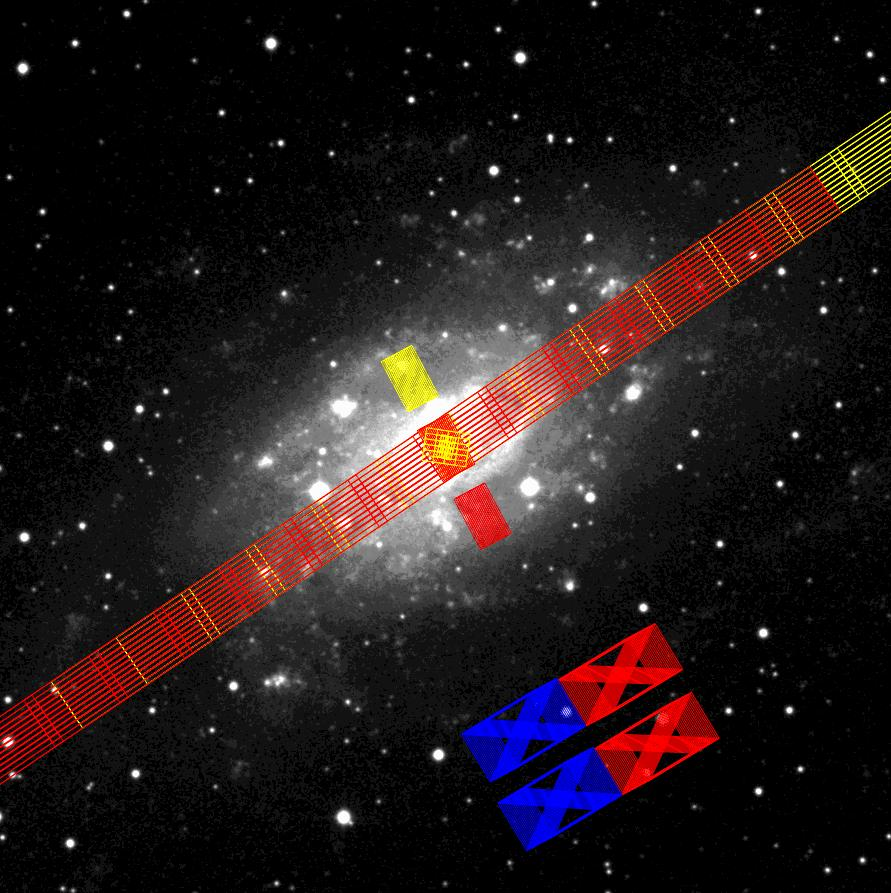
\includegraphics[width=8cm, angle=0]{NGC2403_AORs.jpg}
%\hspace{0.1in}
%\subfigure{text again.\label{figure2}}
%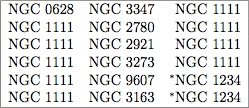
\includegraphics[width=8cm, angle=0]{galaxy_table.jpg}
%\hspace{0.1in}
%\caption{uishdoasdo.\label{figure1}}
%\end{figure}

\subfigure
\centering
%\centerline{\hbox{\hspace{0.0in}
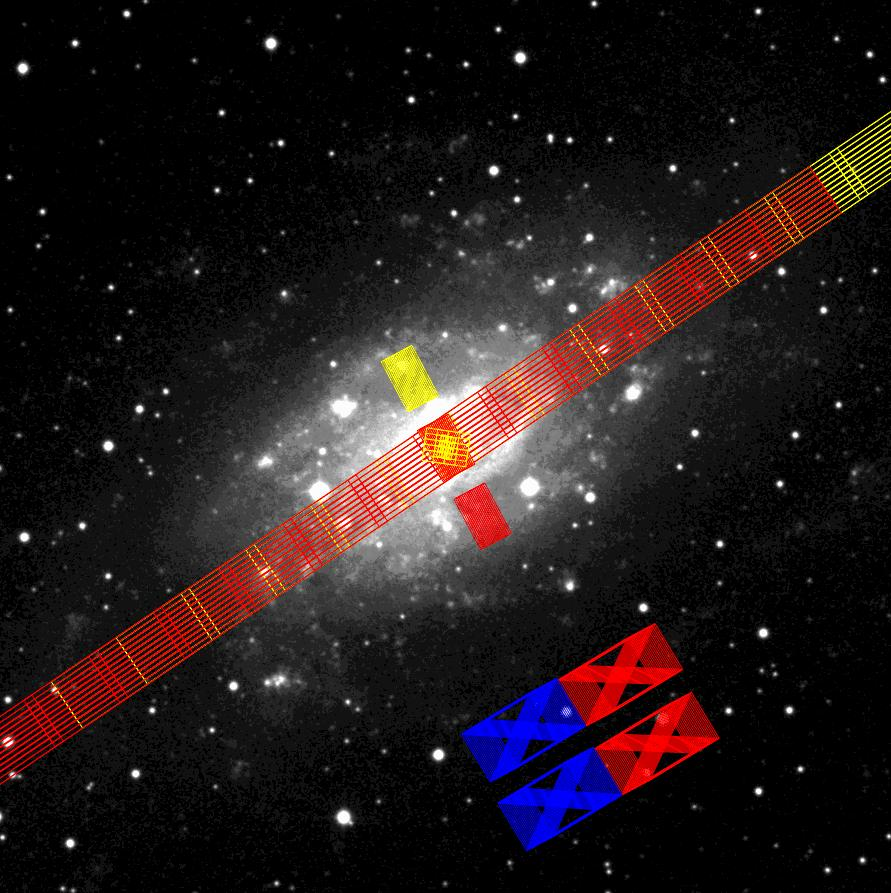
\includegraphics[width=8cm, angle=0]{NGC2403_AORs.jpg}
\hspace{0.1in}
\caption{{\small SINGS IRS spectral mapping footprints for NGC 2403.  The long strip red and yellow strips across the galaxies are the LL1 and LL2 coverage respectively.  The three rectangles across the central region of the galaxy are the SL1 and SL2 observations.  The two smaller sets of footprints over the nucleus are the Spitzer IRS short-high (SH) and long-high (LH) observatios.  SINGS has acquired similar data sets for 65 galaxies, 18 have been observed by BIMA SONG.  SINGS has only studied $\mathrm{H_2}$ for the nuclear regions of each galaxy where the short high (SH), short-low (SL), long-high (LH),� and long-low (LL) observations overlap.  SINGS has not taken advantage of the spectacular IRS LL coverage across the disks of galaxies.  The blue and red boxes in the bottom right of the image are IRS peak up observations.}\label{figure1}}
%\end{figure}


%\begin{table}
%\begin{center}
%\caption{Galaxies for which there are both SINGS and SONG data available.\label{tbl-1}}
%\begin{tabular}{|rrr|}
%\hline
%NGC 0628 & NGC 3347 & NGC 1111\\
%NGC 1111 & NGC 2780 & NGC 1111\\
%NGC 1111 & NGC 2921 & NGC 1111\\
%NGC 1111 & NGC 3273 & NGC 1111\\
%NGC 1111 & NGC 9607 & $\mathrm{^*}$NGC 1234\\
%NGC 1111 & NGC 3163 & $\mathrm{^*}$NGC 1234\\
%\hline
%\end{tabular}
%\caption{{\small Galaxies for which there are both SINGS and SONG data available.  The $\mathrm{^*}$ %denotes a galaxy for which the SINGS LL  data cubes will be available in SINGS data releave 5 (DR 5).  %SINGS LL data cubes are curently available for all other galaxies.}\label{tbl-1}}
%\end{center}
%\end{table}
%{\bf Figure 1}: SINGS IRS spectral mapping footprints for NGC 2403.  The long strip red and yellow strips across the galaxies are the LL1 and LL2 coverage respectively.  The three rectangles across the central region of the galaxy are the SL1 and SL2 observations.  The two smaller sets of footprints over the nucleus are the Spitzer IRS short-high (SH) and long-high (LH) observatios.  SINGS has acquired similar data sets for 65 galaxies, 18 of which have been observed by BIMA SONG.  SINGS has only studied $\mathrm{H_2}$ for the nuclear regions of each galaxy where the short high (SH), long-high (LH), long-low (LL) observations overlap.  SINGS has not taken advantage of the spectacular IRS LL coverage across the disks of galaxies.  The blue and red boxes in the bottom right of the image are IRS peak up observations.


%\begin{figure}[b]
\centerline{\hbox{\hspace{0.0in}
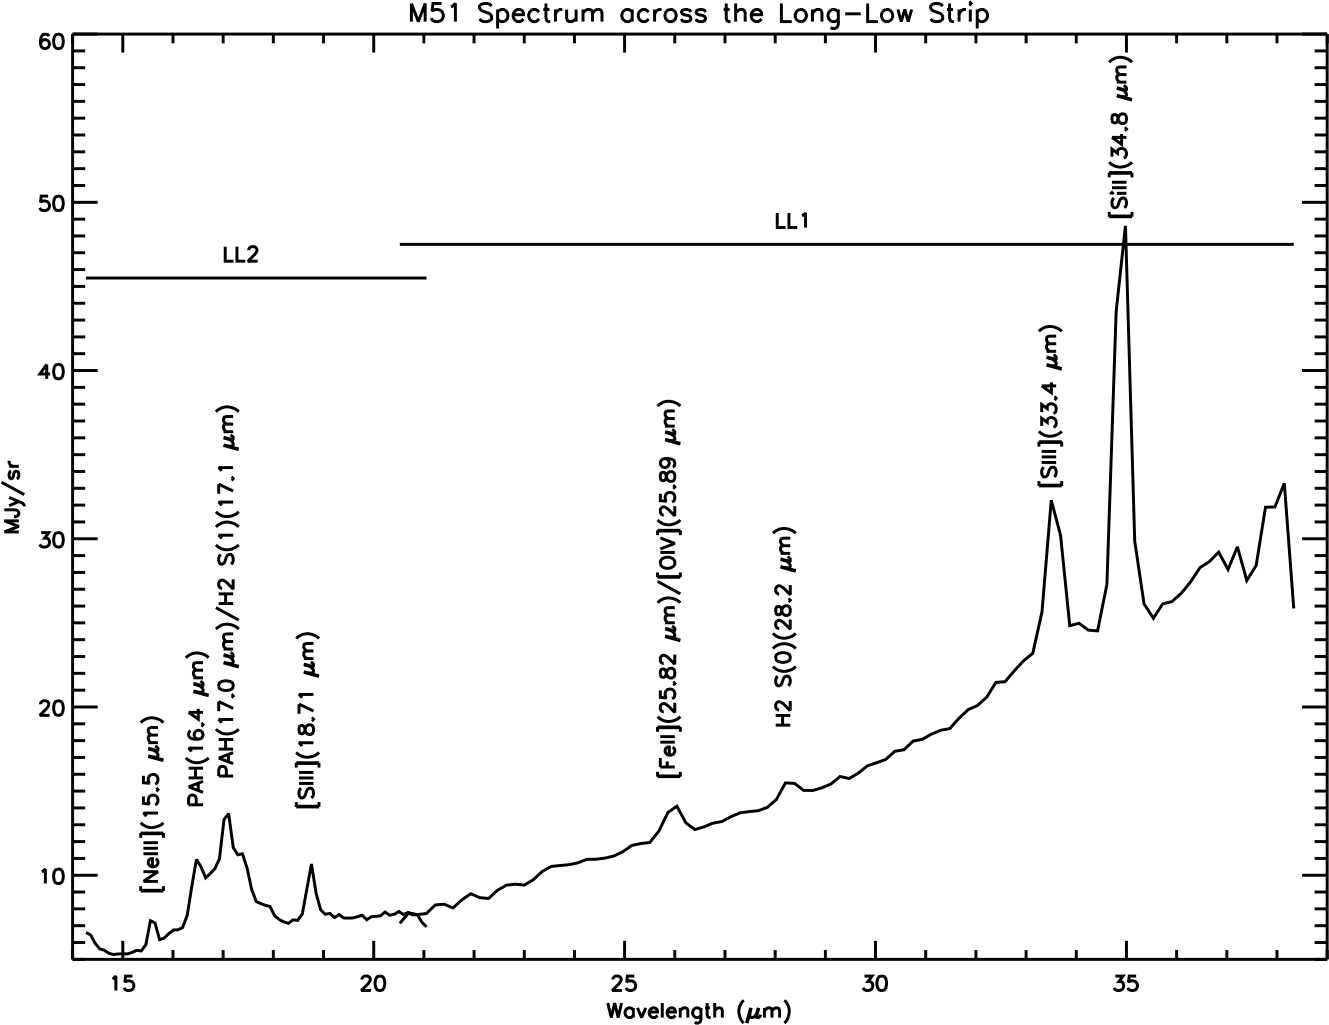
\includegraphics[width=12cm, angle=0]{good_LL_spectrum.jpg}}}
\hspace{0.1in}
%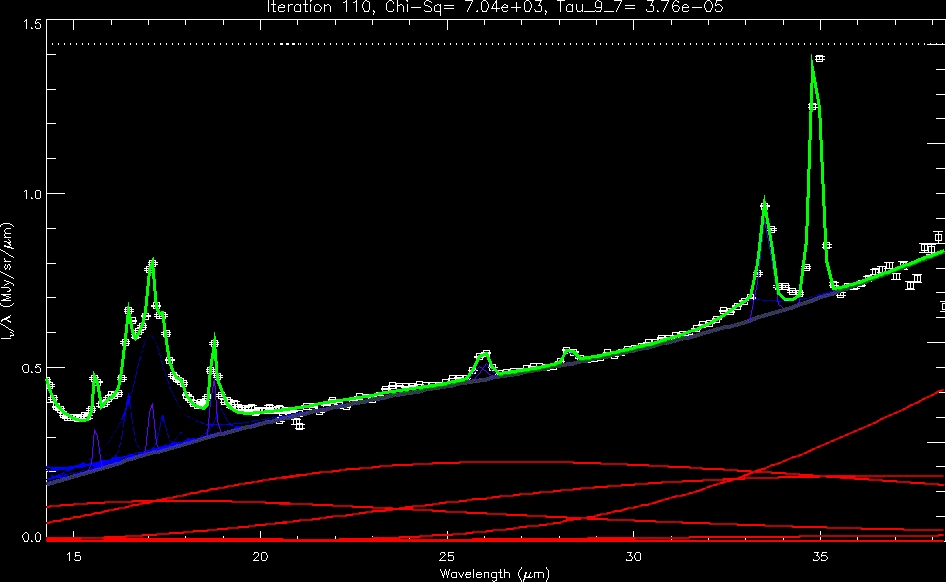
\includegraphics[width=8cm, angle=0]{pahfit.jpg}}}
\caption{{\small A sample LL spectrum taken from the M51 strip (GO -20138) with spectral features noted.  Our study will focus on the $\mathrm{H_2}$ emission across the 18 SINGS LL strips.}
\label{figure2}}

%(b.) We have developed a pipeline that runs PAHFIT across individual spectra in IRS spectral mapping data cubes.  Here we show an example of running PAHFIT on a single spectrum (right).  The green line is the fit to the entire spectrum, the grey line is the fit to the continuum, the blue gaussian-lorentzians are measurements of PAH features, and the purple lines are the gaussian-lorentzian fits to individual spectral lines.}\label{figure2}}
\end{figure}

\clearpage

%We have developed a pipelines that runs PAHFIT across individual spectra in IRS spectral mapping data cubes.  The green line is the fit to the entire spectrum, the grey line is the fit to the continuum, the blue gaussian-lorentzians are measurements of PAH features, and the purple lines are the gaussian-lorentzian fits to individual spectral lines.
%\label{figure3}}
%\end{figure}

\begin{figure}
\subfigure
\centering
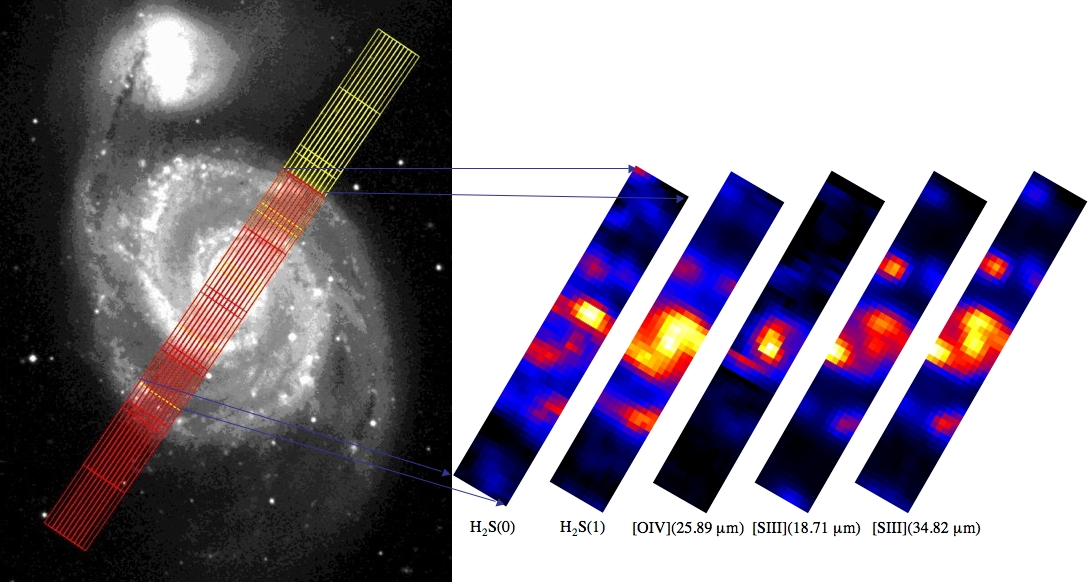
\includegraphics[width=17.5cm, angle=0]{m51maps.jpg}}}
\hspace{0.5in}
\caption{{\small Shown are the IRS LL spectral mapping AORs for M51a (GO - 20138).  Maps of the individual lines were created with our PAHFIT pipeline allowing for us to determine the flux of al lines from 14 - 38 $\mu$m in the LL data cube.  Shown are the maps of the $\mathrm{H_2}$ S(0) (28.2 $\mu$m), $\mathrm{H_2}$ S(1) (17.1 $\mu$m), [OIV](25.89 $\mu$m), [SIII](18.71 $\mu$m), and [SIII](33.82 $\mu$m) lines.}\label{figure3}}\\

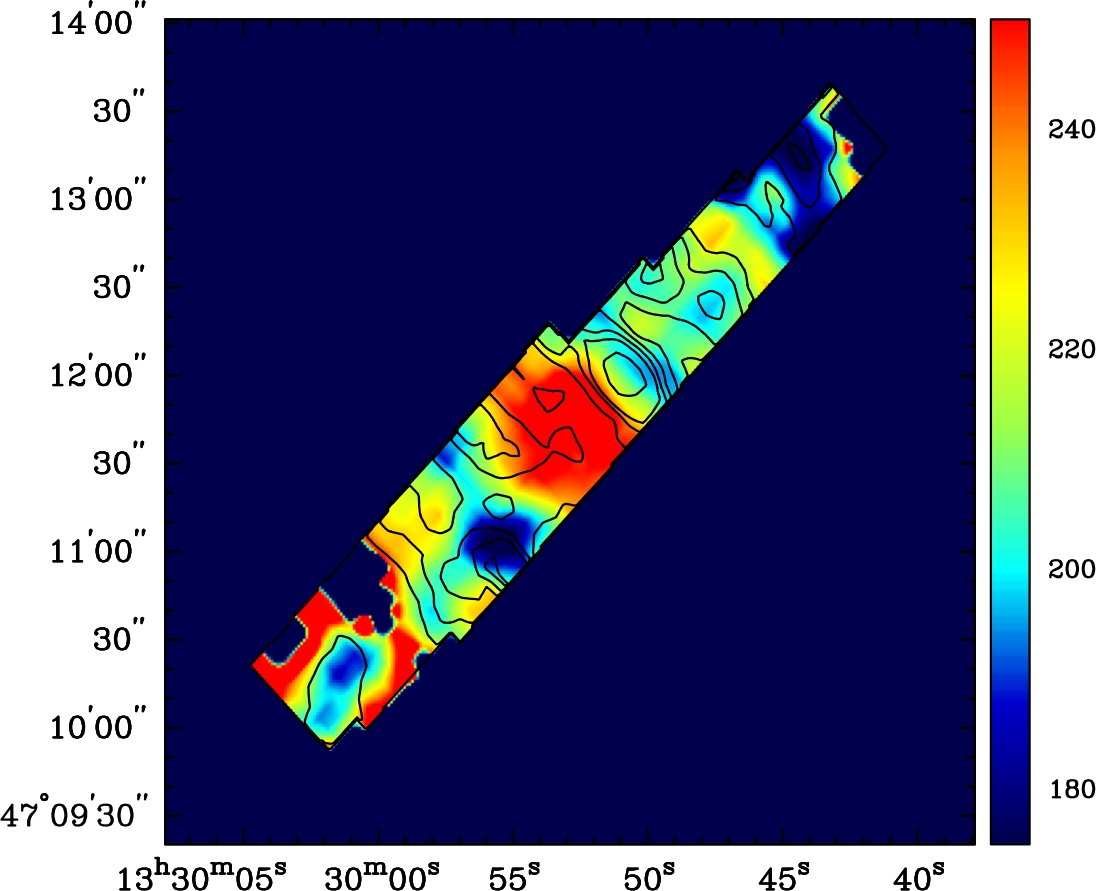
\includegraphics[width=9cm, angle=0]{color_temp_mass_cold.jpg}
\hspace{0.1in}
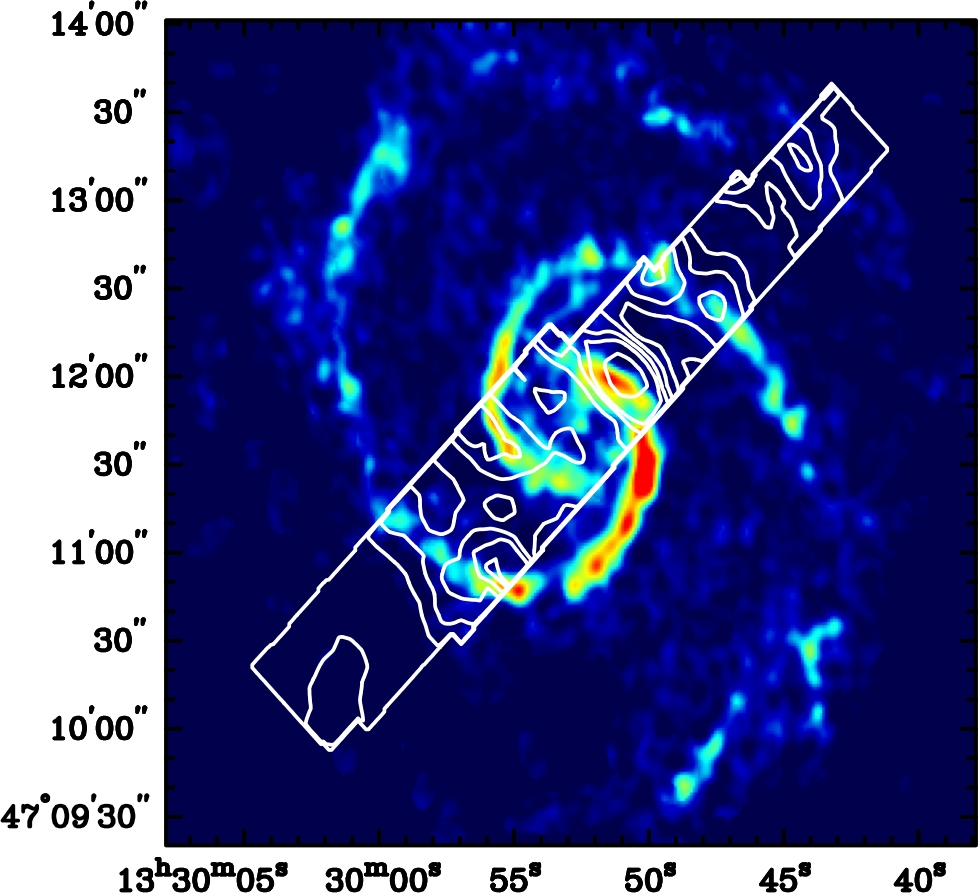
\includegraphics[width=8cm, angle=0]{proposal_co_v_h2.jpg}}}
\caption{{\small $Left$: Map of the warm (T = 100 - 300) mass distribution (in contours) plotted over the excitation temperature distribution (in color).  The temperature distribution is in units of Kelvin; the contours are spaced at .... $\mathrm{M_{sun}}$/$\mathrm{pc^2}$.  $Right$: Comparison of the warm $\mathrm{H_2}$ mass to the cold (T = 5 - 10 K) $\mathrm{H_2}$ that is traced by CO (J - 1 - 0) emission. The contours are the same as in the plot on the $left$.  The map is in units of ...   The CO map of M51 was obtained by the BIMA SONG.}\label{figure4}}



\end{figure}


\clearpage

\section{References}
\\
Brunner et al., 2007, submitted\\
Helfer et al.,  2003, ApJS, 145, 259\\
Higdon et al., 2006, ApJ, 648, 323\\
Kennicutt et al., 2003, PASP, 115, 928\\
Lutz et al., 1998, A&A, 333, L75\\
Regan et al., 2001, ApJ, 561, 218\\
Rigopoulou et al., 2002, A&A, 389, 374\\
Roussel et al., 2007, TBD\\
Sheth et al., 2000, ApJ, 532, 221 \\
Smith et al., 2004, ApJS, 154, 199\\
Smith et al., 2007, ApJ, accepted (currently on astro-ph/0610913)\\
Schaerer and Stasinska, 1999, A&A, 345, L17\\
Vogel et al., 1988, $Nature$, 334, 402\\
Young and Deveraux, 1991, ApJ, 373, 414\\

\section{Brief Resume/Bibliography}

{\bf PI}:  Gregory Brunner is a graduate student at Rice University  and a 2006-2007 Spitzer Visiting Graduate Student Fellow.  During the fellowship he worked with Kartik Sheth on IRS spectral mapping data of M51a.  He has developed a pipeline that takes IRS low resolution data cubes and creates line flux maps of every spectral feature in the data cube.  He is currently working on submitting a draft of the results of a study of the $\mathrm{H_2}$ emission, excitation, and mass across M51a that he completed during the Spitzer Visiting Graduate Student Fellowship.\\

{\bf Co-I}: Reginald Dufour is a professor in the Department of Physics and Astronomy at Rice University.  His interests are observational astrophysics of planetary nebulae, HII regions, and galaxies.\\

{\bf Co-I}: Kartik Sheth is a research scientist at Spitzer Science Center and a member of the Spitzer IRS instrument team.\\

{\bf Co-I}: Stuart Vogel is a professor of astronomy and the director of the lab for millimeter-wave astronomy at the University of Maryland.  His main research interests are star formation and galaxy evolution.\\

{\bf Co-I}: Mark Wolfire is a research scientist at the University of Maryland.  He is an expert on modeling photo-dissociation regions.\\
\\
{\bf Selected references relevant to this proposal from the team:}\\
\\
 Brunner et al. 2007, submitted\\
 Dufour, R.J. et al.\\
 Dufour, R.J. et al.\\
 Dufour, R.J. et al.\\
 Sheth, K. et al., 2000, ApJ, 532, 221\\
 Sheth, K. et al., 2002, AJ, 124, 2581\\
 Sheth, K. et al., 2004, ApJL, 614, 5\\
 Vogel, S.N. et al., 1993, PASP, 105, 666\\
 Vogel, S.N. et al., 1988, $Nature$, 334, 402\\
 Wolfire, M. et al., 2003, ApJ, 586, 278\\
 Wolfire, M. et al., 1995, ApJ, 443, 152\\

\section{Status of Existing Spitzer Programs}


This section should provide the status of any Spitzer programs 
(observing or AR/TR) on which the PI or ANY of the CoIs are PI
or technical contact (TC). This section should NOT have any 
figures. This section should NOT provide a comprehensive history 
of every Spitzer program in which you have EVER been involved. 
If you have more than 5 programs, you may just provide a 
summary paragraph. If you feel a list of your 10 most recent 
Spitzer publications really MUST be included, put them here.\\

{\bf Co-I} R. Dufour is a Co-I on GO - 3412, GO - 20049, and GO - 20057.  What is the status Reggie?\\

{\bf Co-I} K.\ Sheth is the PI for GO - 20138 and Co-I on GO - 20587.  The
data for program #20138 has been reduced and analyzed and is in preparation for publication.  The data for program #20587 has been reduced and is currently under analysis.\\

{\bf Co-I} S.\ Vogel is a Co-I on Go - 20138 and GO - 20587. \\

{\bf Co-I} M. Wolfire is ... 

\section{Financial Contact Information}

Provide the contact information for the appropriate person in
the  institution's Sponsored Research Office (or equivalent) for
the PI and Co-I's that require funding support.\\

For PI G. Brunner and Co-I R. Dufour\\
Alice Example\\
example@caltech.edu\\
Rice University\\
Mail Code 11 - 2\\
Houston, TX 77005\\
phone\\
\\
For Co-I K. Sheth\\
Eloise Kennedy\\
eks@ipac.caltech.edu\\
Image Processing and Analysis Center\\
MS-220-6\\
Pasadena, CA 91125\\
626.395.1801\\
\\
For Co-Is S. Vogel and M. Wolfire\\
Monique Anderson, Contract Manager\\
manderson@umresearch.umd.edu\\
University of Maryland, College Park\\
3112 Lee Building\\
College Park, MD 20742\\
301.405.6272\\

\section{Cost Plan and Budget Narrative}

Put the descriptive budget narrative here. It should describe 
how the funds will be allocated. There is no page limit to the 
narrative. Fill in the cost plan table (Spitzer Cycle-4 Budget).

Cost plans are limited to one year duration (for Cycle-4: Oct 
2007 - Sep 2008) and the funds must be used within 2 years of 
the award.

Archival and Theoretical Research proposers must send three 
paper copies of the institutionally endorsed cost plan and 
narrative to the SSC by Friday, February 24 2007, 5:00 pm (PST). 

The Spitzer Science Center's postal mailing address is:\\
Spitzer Science Center\\
California Institute of Technology\\
Mail Code 314-6\\
1200 East California Boulevard\\
Pasadena, CA 91125\\
USA\\

\clearpage
\begin{table}[ht]
\caption{Spitzer Cycle-4 Budget 1 Oct 2007 -- 30 Sep 2008}
\begin{tabular}{|l|l|l|l|l|}
\hline
Narrative & & & & \\
\hline
Footnote & Cost Element & & & \\
\hline
\hline
 & Direct Labor Hours (by labor category) & Hours & Rate & Amount\\
\hline
 & & & & \\
\hline
 & & & & \\
\hline
 & & & & \\
\hline
 & & & & \\
\hline
 & & & & \\
\hline
 & & & & \\
\hline
 & & & & \\
\hline
 & Total Direct Labor & & & \\
\hline
\hline
 & Overhead & Base & Rate & \\
\hline
 & & & & \\
\hline
 & & & & \\
\hline
 & & & & \\
\hline
 & & & & \\
\hline
 & & & & \\
\hline
 & & & & \\
\hline
 & & & & \\
\hline
 & Total Overhead & & & \\
\hline
\hline
 & Material Costs & & & \\
\hline
 & Material Burden & & & \\
\hline
 & Total Material & & & \\
\hline
\hline
 & Subcontract Cost & & & \\
\hline
 & Subcontract Burden & & & \\
\hline
 & Total Subcontract & & &\\
\hline
\hline
 & Other Direct Cost (ODC) & & & \\
\hline
 & & & & \\
\hline
 & & & & \\
\hline
 & & & & \\
\hline
 & & & & \\
\hline
 & & & & \\
\hline
 & Total ODC & & & \\
\hline
\hline
 & Sub-Total Cost & & & \\
\hline
 & Total General \& Administrative & & & \\
\hline
 & Total Cost & & & \\
\hline
\end{tabular}
\end{table}

\end{document}